\section{\hspace{1em}Въведение}

\begin{frame}[t]{Термини от епидемиологията}
  \begin{itemize}
    \item Патоген е причинител на зараза (напр. вирус, бактерия, прион).
    \item Вектор е носител на патоген, който може да зарази други индивиди.
    \item S (Susceptible - Податливи) - податливи са тези, които не носят патогена и могат да бъдат заразени с него
    \item I (Infected - Заразени) - заразени са носители на патогена
    \item Заболяване има ендемичен характер, когато има (приблизително) константен ненулев брой заразени.
  \end{itemize}
\end{frame}

\begin{frame}[t]{Малария}
  Симптоми са периодичен пароксизъм(продължителни спазми, потене, треска), умора, главоболие, хепатомегалия (разраснал се черен дроб), белодробен оток, анемия (намалено количество еритроцити), мозъчек оток, смърт.

  Патогенът е един 4 вида от рода \textit{Plasmodium} маларийни плазмодии, които са едноклетъчни еукариоти, т.е. едноклетъчни с ядро. Интензивността на симптомите зависи от вида плазмодий.

  В края на XIX век Ronald Ross доказва, че вектора на маларията са комарите от род \textit{Anopheles}.
  В началото на XX век моделира маларията с две диференциални уравнения, като модела му е основа за моделирането на векторнопредавани заболявания и до днес.
\end{frame}

\begin{frame}[t]{Разпространение на маларията}
  Хората могат да оздравеят, като организмът им се прочисти от плазмодиите.
  Не развиват траен имунитет, но обикновено повторни заболявания се претърпяват по-лесно.

  Комарите са насекоми и нямат имунна система, така че не могат да се предпазват от паразити.

  Затова в моделите на Ross динамиката се описва чрез прехода между класове:
  \begin{itemize}
    \item $S \rightarrow I \rightarrow S$ (SIS) при хората
    \item $S \rightarrow I$ (SI) при комарите
  \end{itemize}

  \begin{figure}
    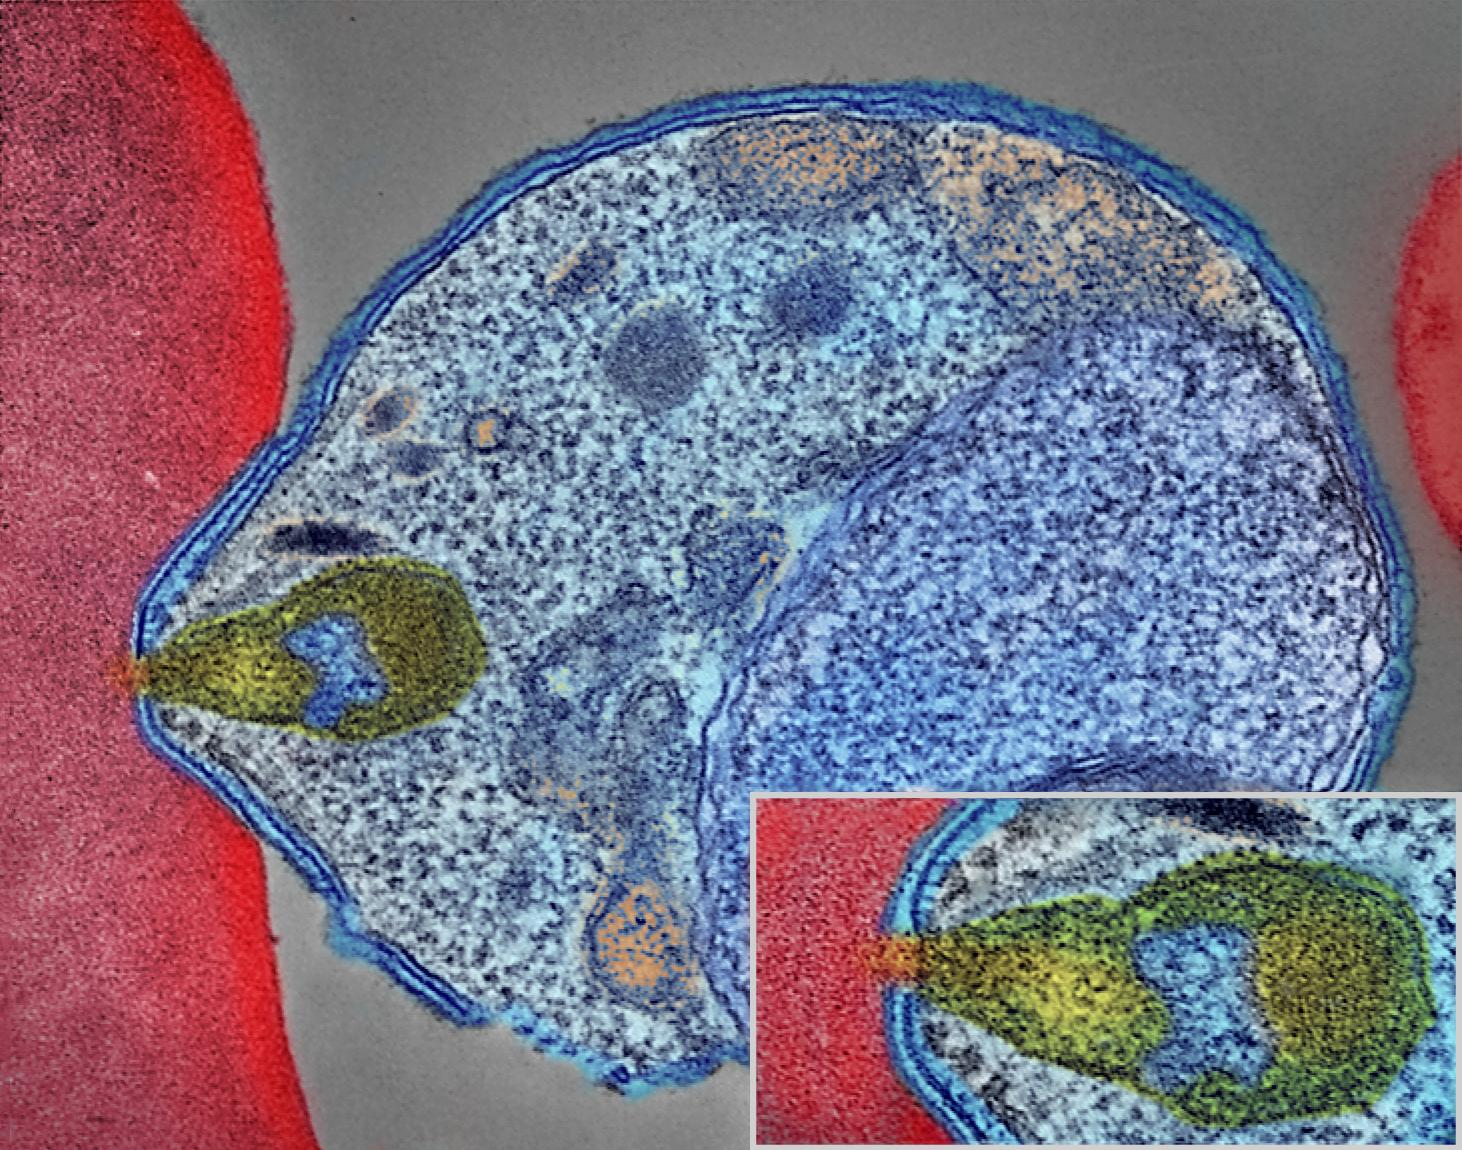
\includegraphics[height=0.3\textheight]{Malaria_Parasite_Connecting_to_Human_Red_Blood_Cell_(34034143483).jpg}
    \centering
    \caption{Оцветена снимка от електронен микроскоп на плазмодий нападащ еритроцит}
  \end{figure}
\end{frame}

\begin{frame}[t]{Краен вид на Хамилтонияна}
  \begin{footnotesize}
    \begin{multline*}
      \label{eq:HamiltonianShort}
      \mathcal{H}(\boldsymbol{z}, \grad{v}) = \\
      \left[\gamma_1 x_1 - (1-x_1) \left(b_{11} y_1 + b_{12} y_2\right) \right] \pdv{v}{x_1} +
      \left[\gamma_2 x_2 - (1-x_2) \left(b_{21} y_1 + b_{22} y_2\right) \right] \pdv{v}{x_2} + \\
      \left[\mu_1 y_1 - (1-y_1) \left(c_{11} x_1 + c_{12} x_2\right) \right] \pdv{v}{y_1} +
      \left[\mu_2 y_2 - (1-y_2) \left(c_{21} x_1 + c_{22} x_2\right)\right] \pdv{v}{y_2} + \\
      \max\bigg\{0, \kappa \bar{u}_1 (1-x_1) \left(b_{11} y_1 + b_{12} y_2\right) \pdv{v}{x_1} + c_{11} \kappa \bar{u}_1 x_1 (1-y_1)\pdv{v}{y_1} + c_{21} \bar{u}_1 x_1 (1-y_2) \pdv{v}{y_2}
      \bigg\} + \\
      \max\bigg\{0, \kappa \bar{u}_2 (1-x_2) \left(b_{21} y_1 + b_{22} y_2\right) \pdv{v}{x_2} + c_{12} \bar{u}_2 x_2 (1-y_1)\pdv{v}{y_1} + c_{22}  \bar{u}_2 x_2 (1-y_2)\pdv{v}{y_2} \bigg\}
    \end{multline*}

  \end{footnotesize}
\end{frame}
